% Chapter Template

\chapter{2-D Memristor Simulation} % Main chapter title

\label{Chapter6} % Change X to a consecutive number; for referencing this chapter elsewhere, use \ref{ChapterX}

\lhead{Chapter 6. \emph{Memristor Simulation}} % Change X to a consecutive number; this is for the header on each page - perhaps a shortened title

\section{Effect of PEDOT:PSS Thickness}
\section{2-D Memristor Simulation Using a Pulse Train}

\begin{figure}[!htp]
\centering
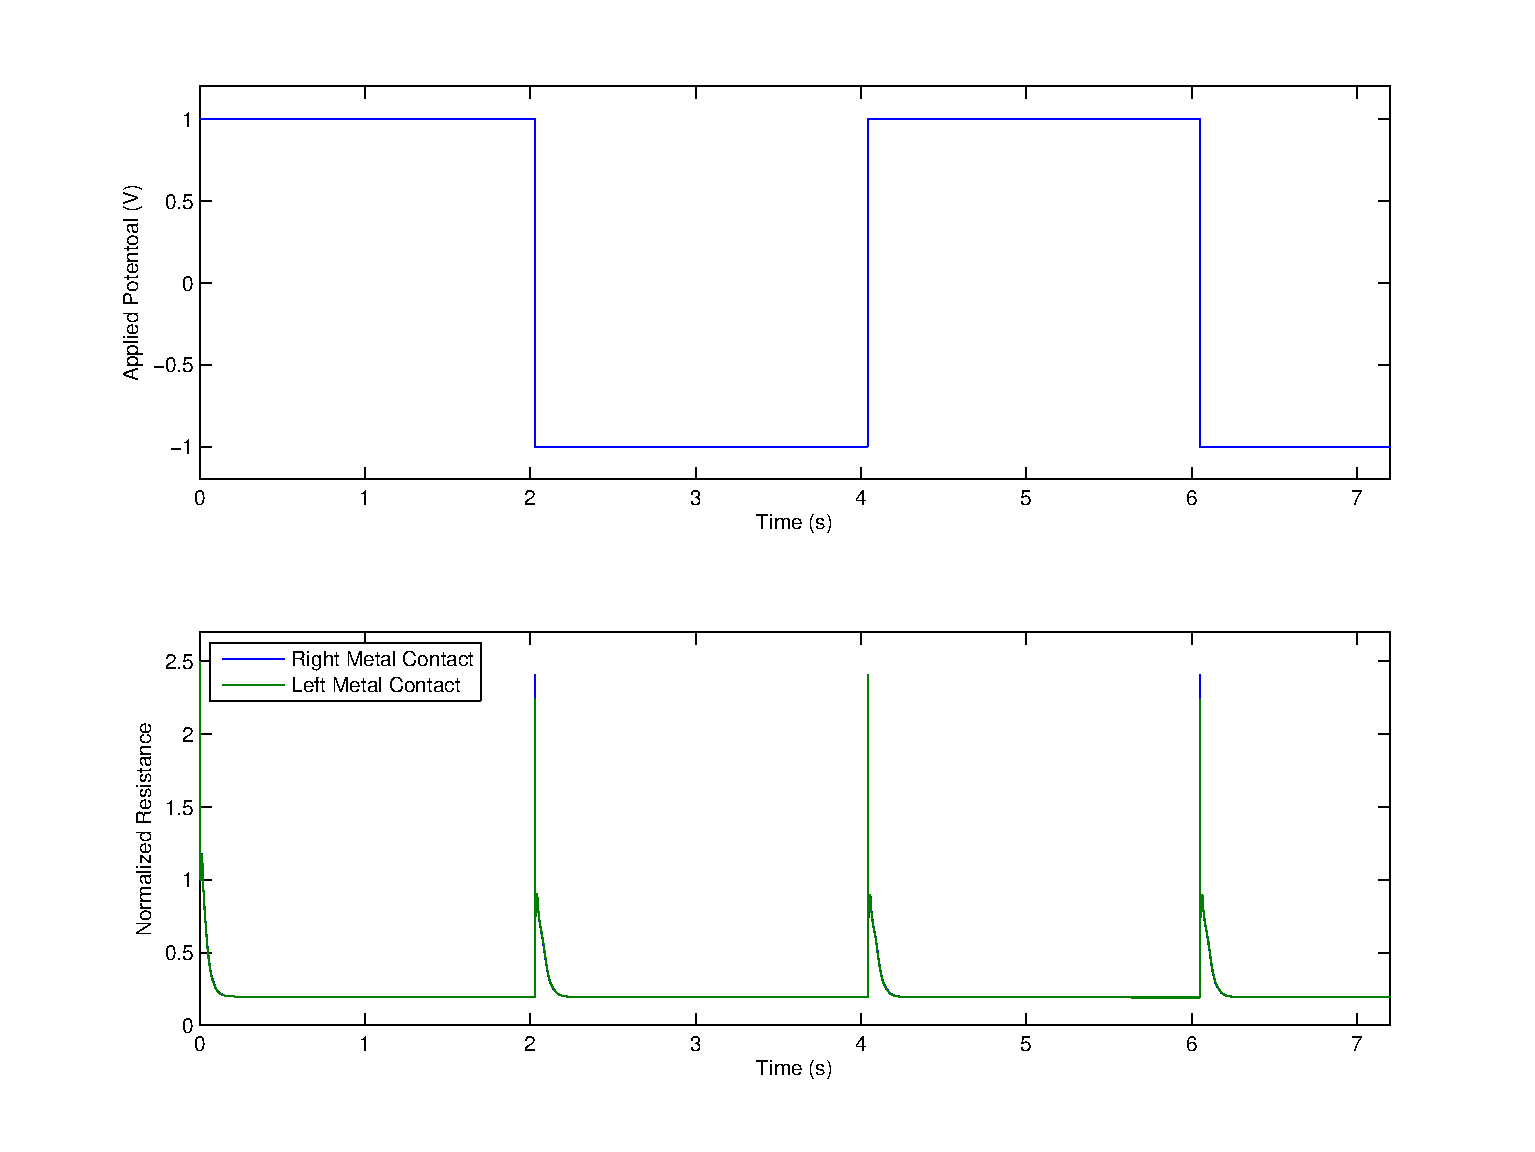
\includegraphics[scale=0.50]{2D_Memristor_Pulse_Train}
\caption{} 
\label{}
\end{figure}


\begin{figure}[!htp]
\centering
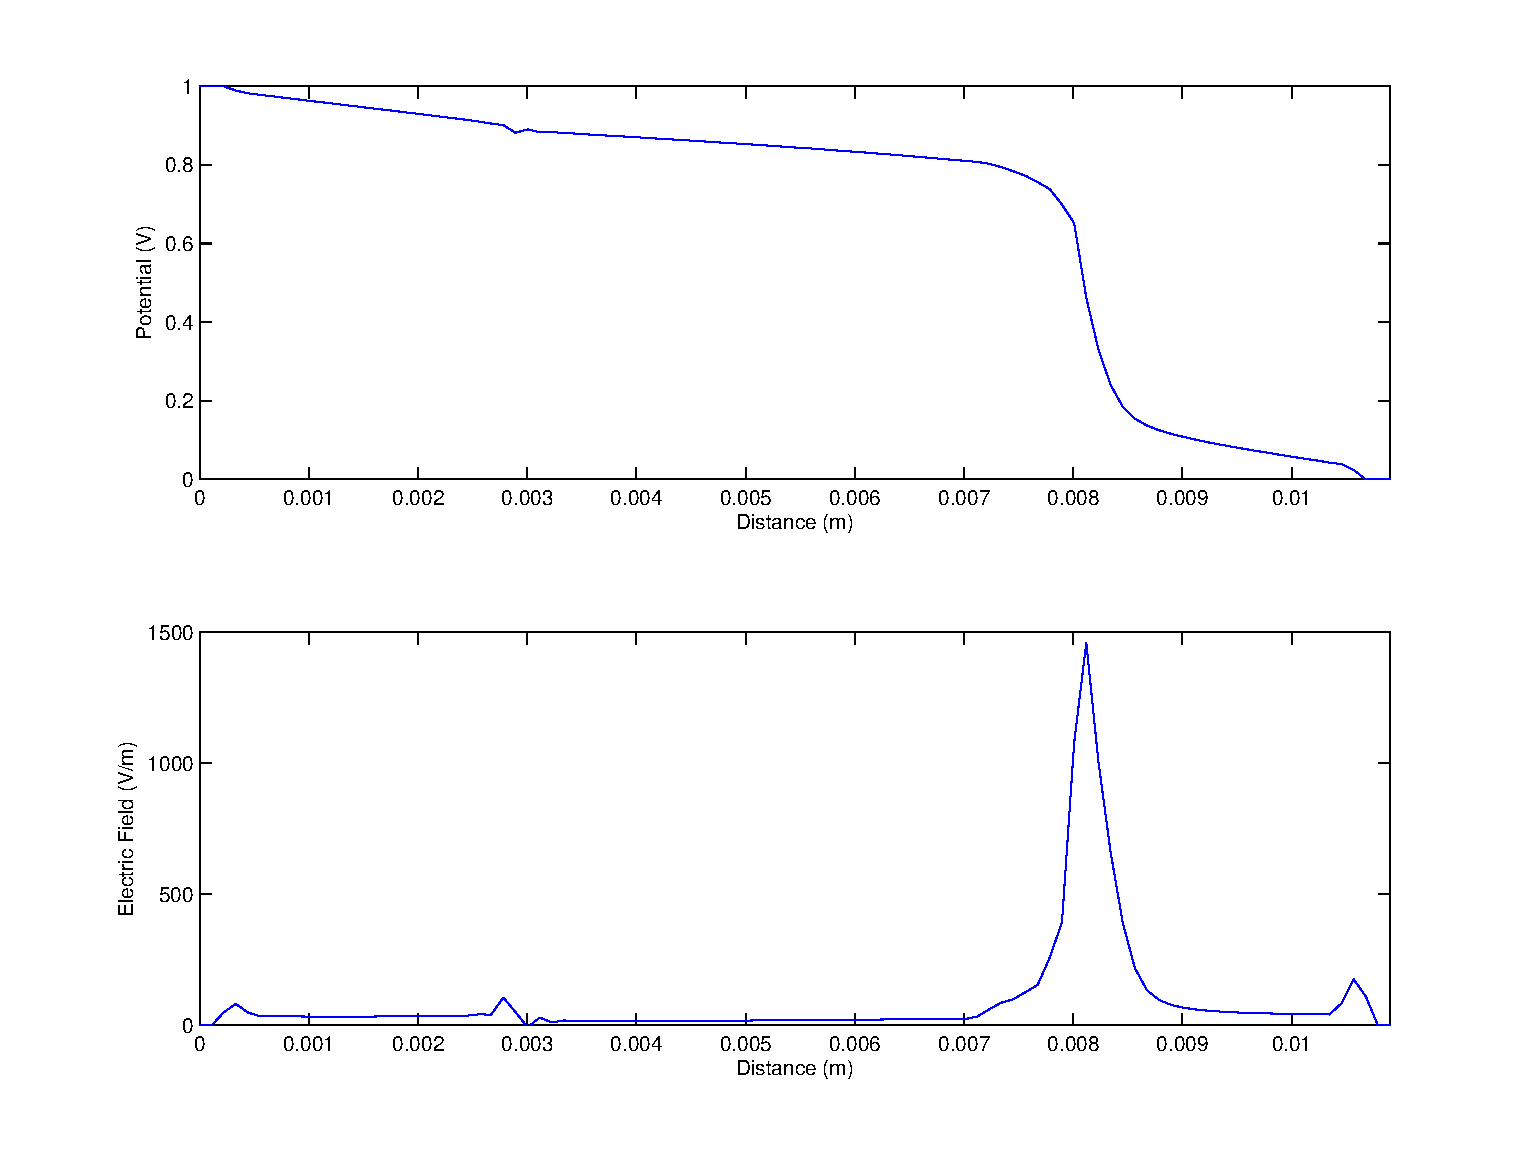
\includegraphics[scale=0.50]{2D_Memristor_Pulse_Train_EV}
\caption{} 
\label{}
\end{figure}

\begin{figure}[!htp]
\centering
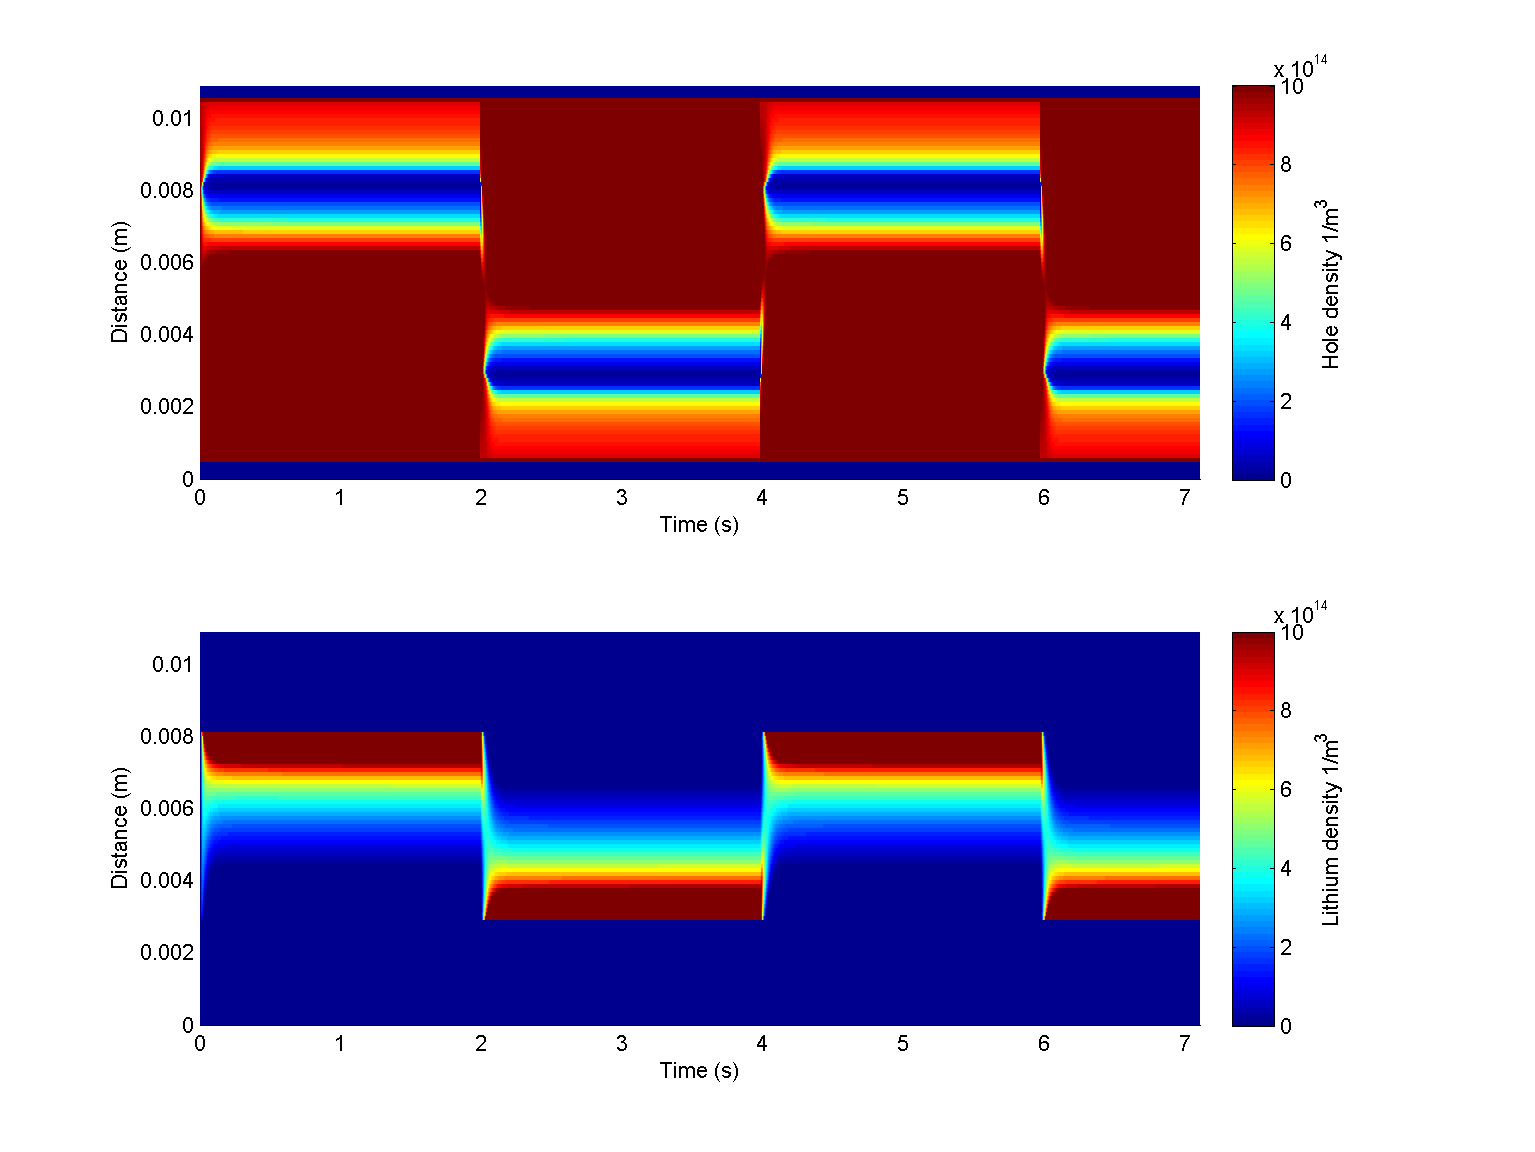
\includegraphics[scale=0.50]{2D_Memristor_Pulse_Lithium_Hole}
\caption{} 
\label{}
\end{figure}

\begin{figure}[!htp]
\centering
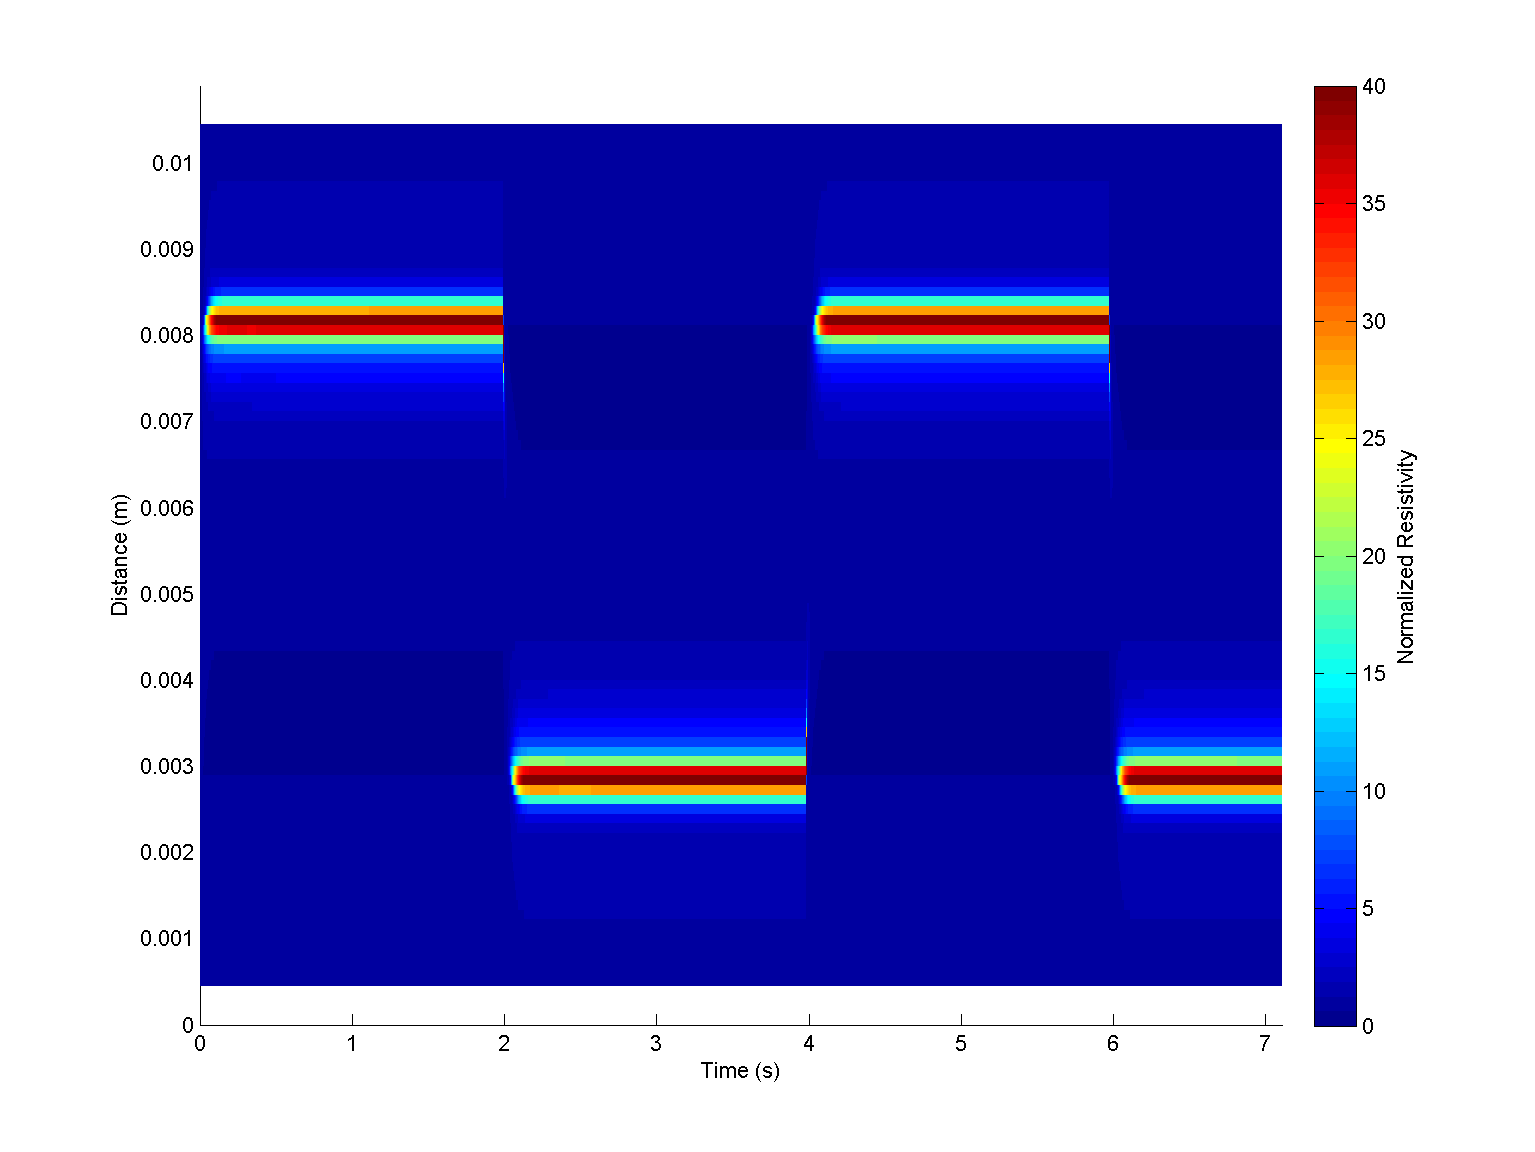
\includegraphics[scale=0.50]{2D_Memristor_Resistivity}
\caption{} 
\label{}
\end{figure}

\begin{figure}[!htp]
\centering
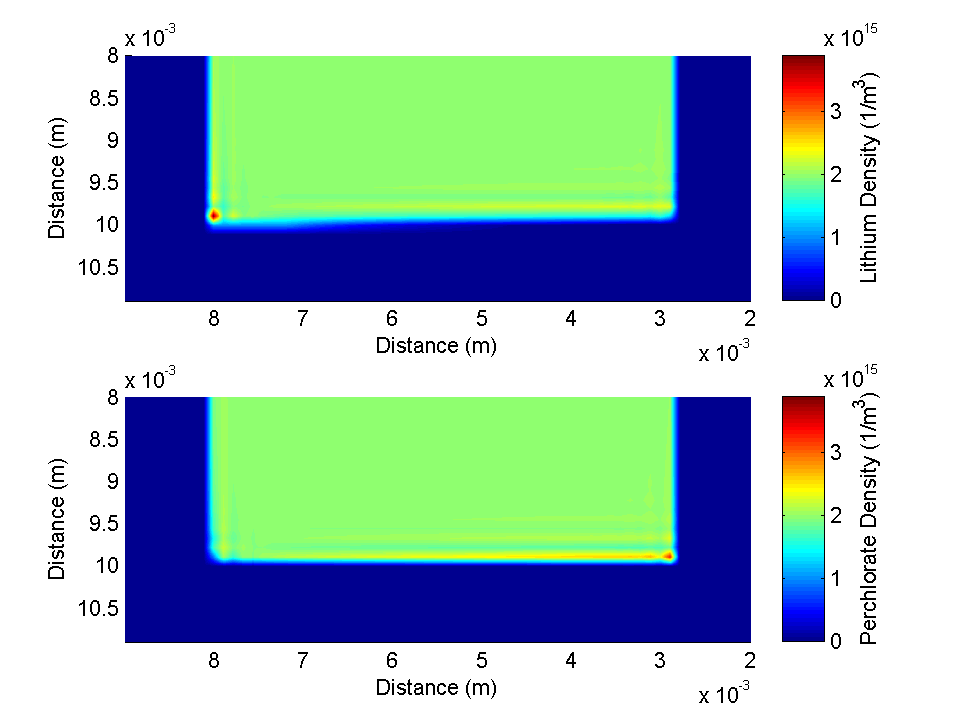
\includegraphics[scale=0.70]{2D_Memristor_Pulse_Train_2_Lithium_Perchlorate}
\caption{} 
\label{}
\end{figure}

\begin{figure}[!htp]
\centering
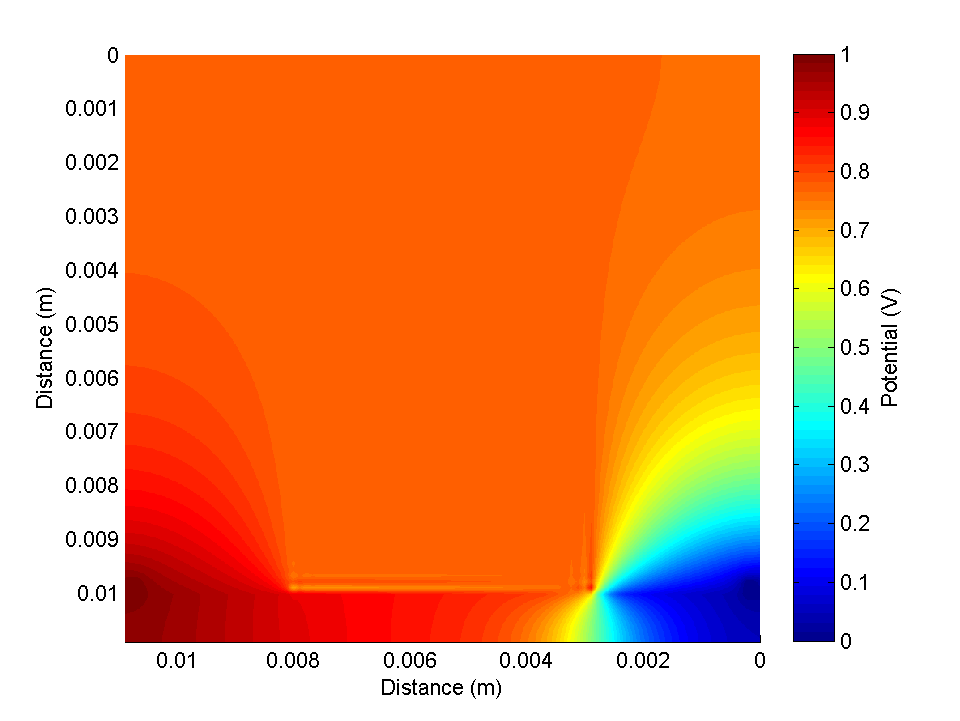
\includegraphics[scale=0.70]{2D_Memristor_Pulse_Train_2DV}
\caption{} 
\label{}
\end{figure}

\begin{figure}[!htp]
\centering
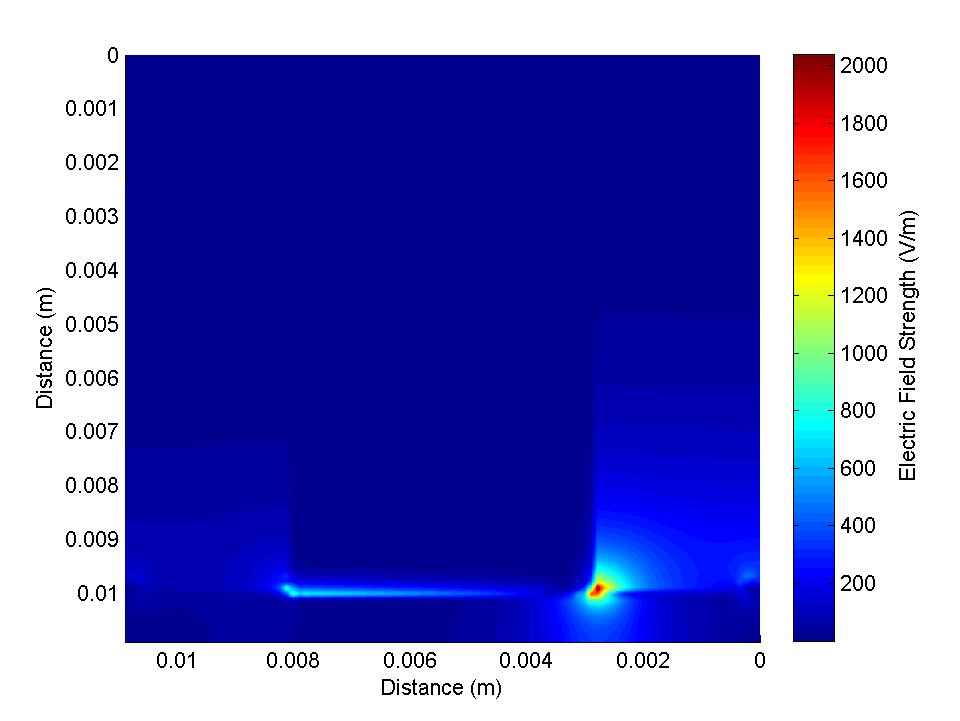
\includegraphics[scale=0.70]{2D_Memristor_Pulse_Train_2DE}
\caption{} 
\label{}
\end{figure}


\begin{figure}[!htp]
\centering
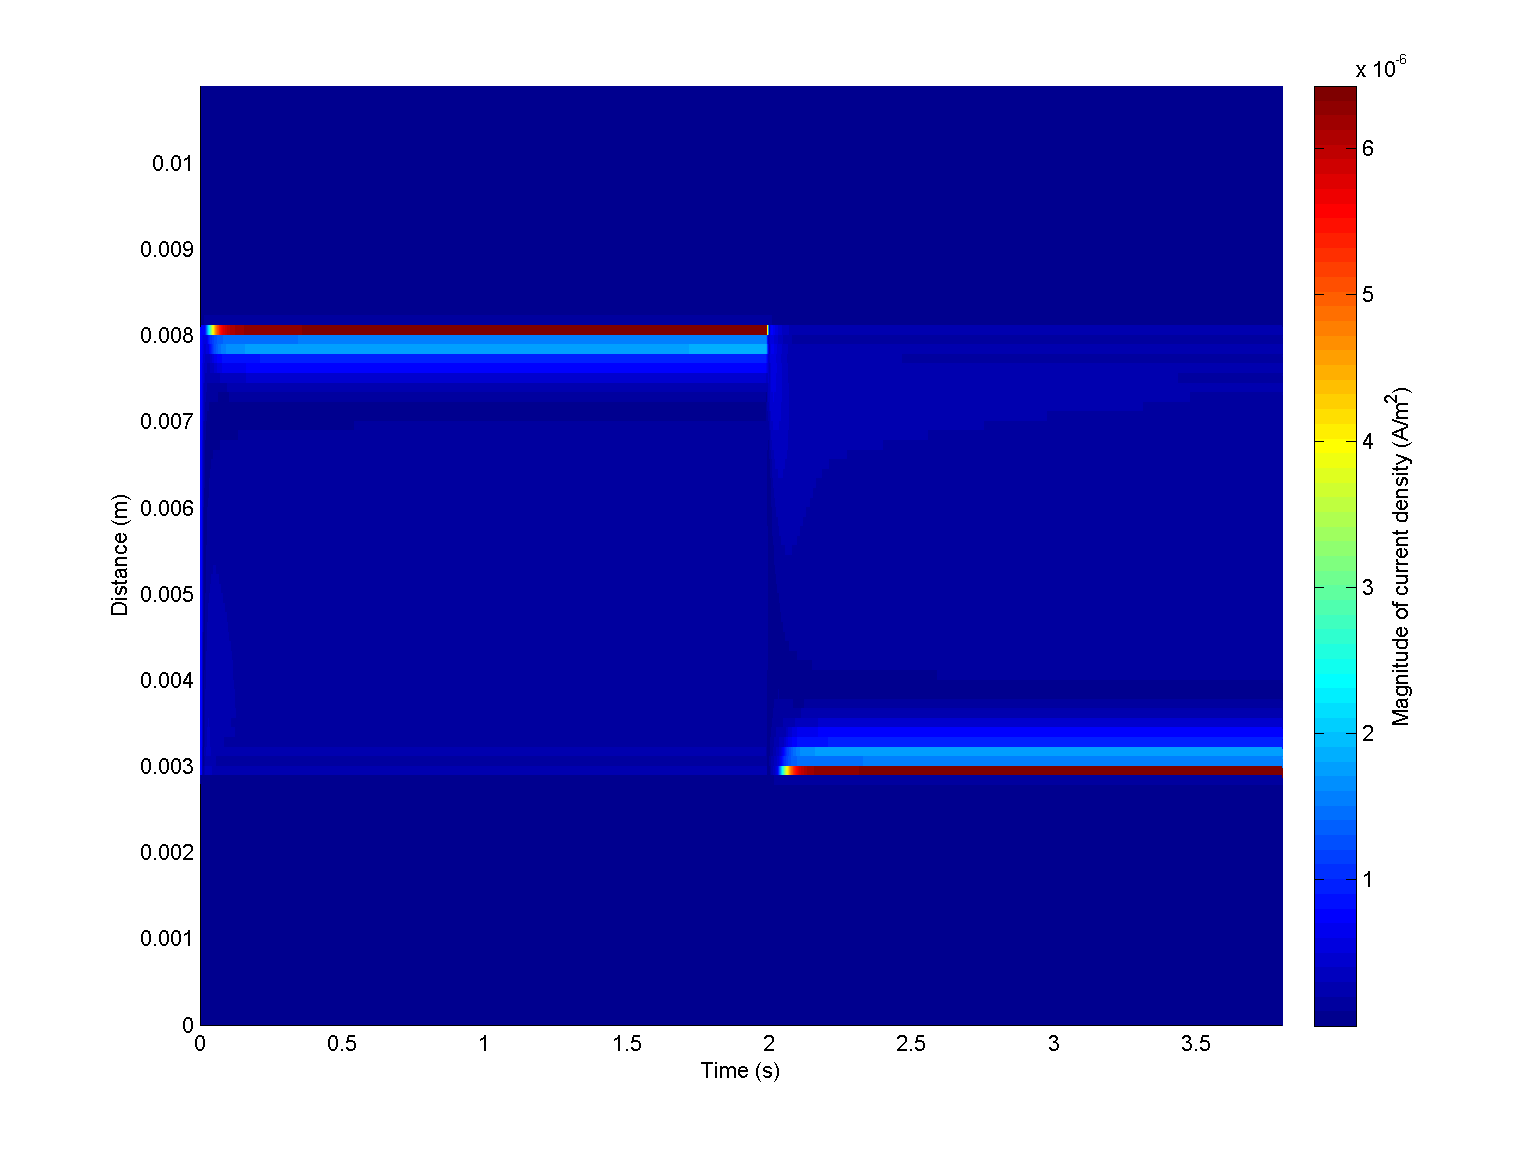
\includegraphics[scale=0.50]{2D_Memristor_Pulse_Lithium_J}
\caption{} 
\label{}
\end{figure}


\clearpage
\section{2-D Memristor Simulation Using a Sinusoid}

\begin{figure}[!htp]
\centering
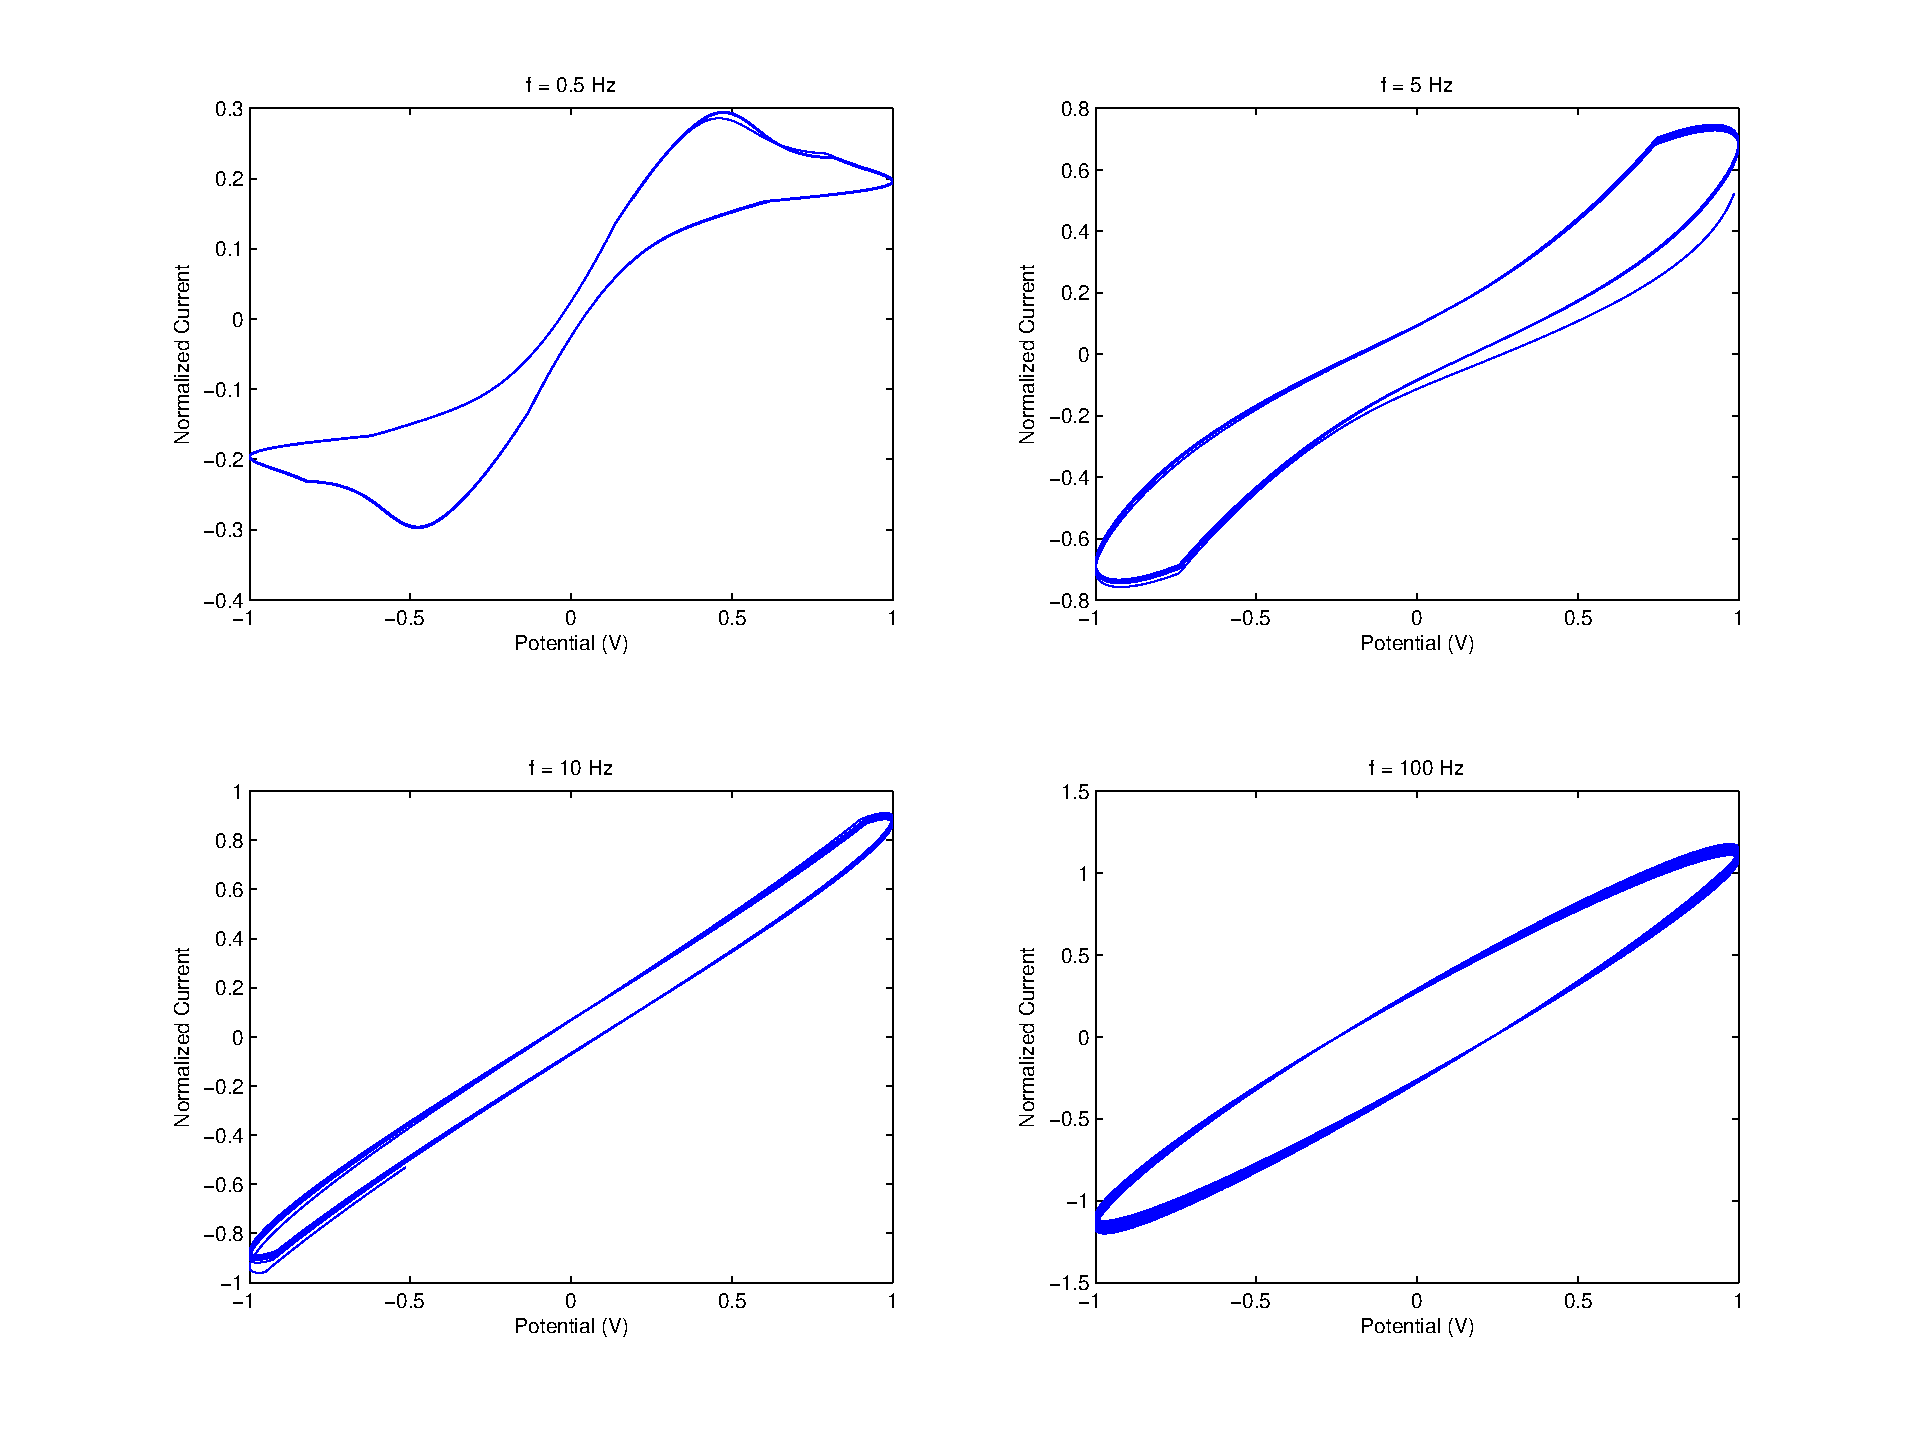
\includegraphics[scale=0.45]{2D_Memristor_bowtie_f}
\caption{} 
\label{}
\end{figure}


\begin{figure}[!htp]
\centering
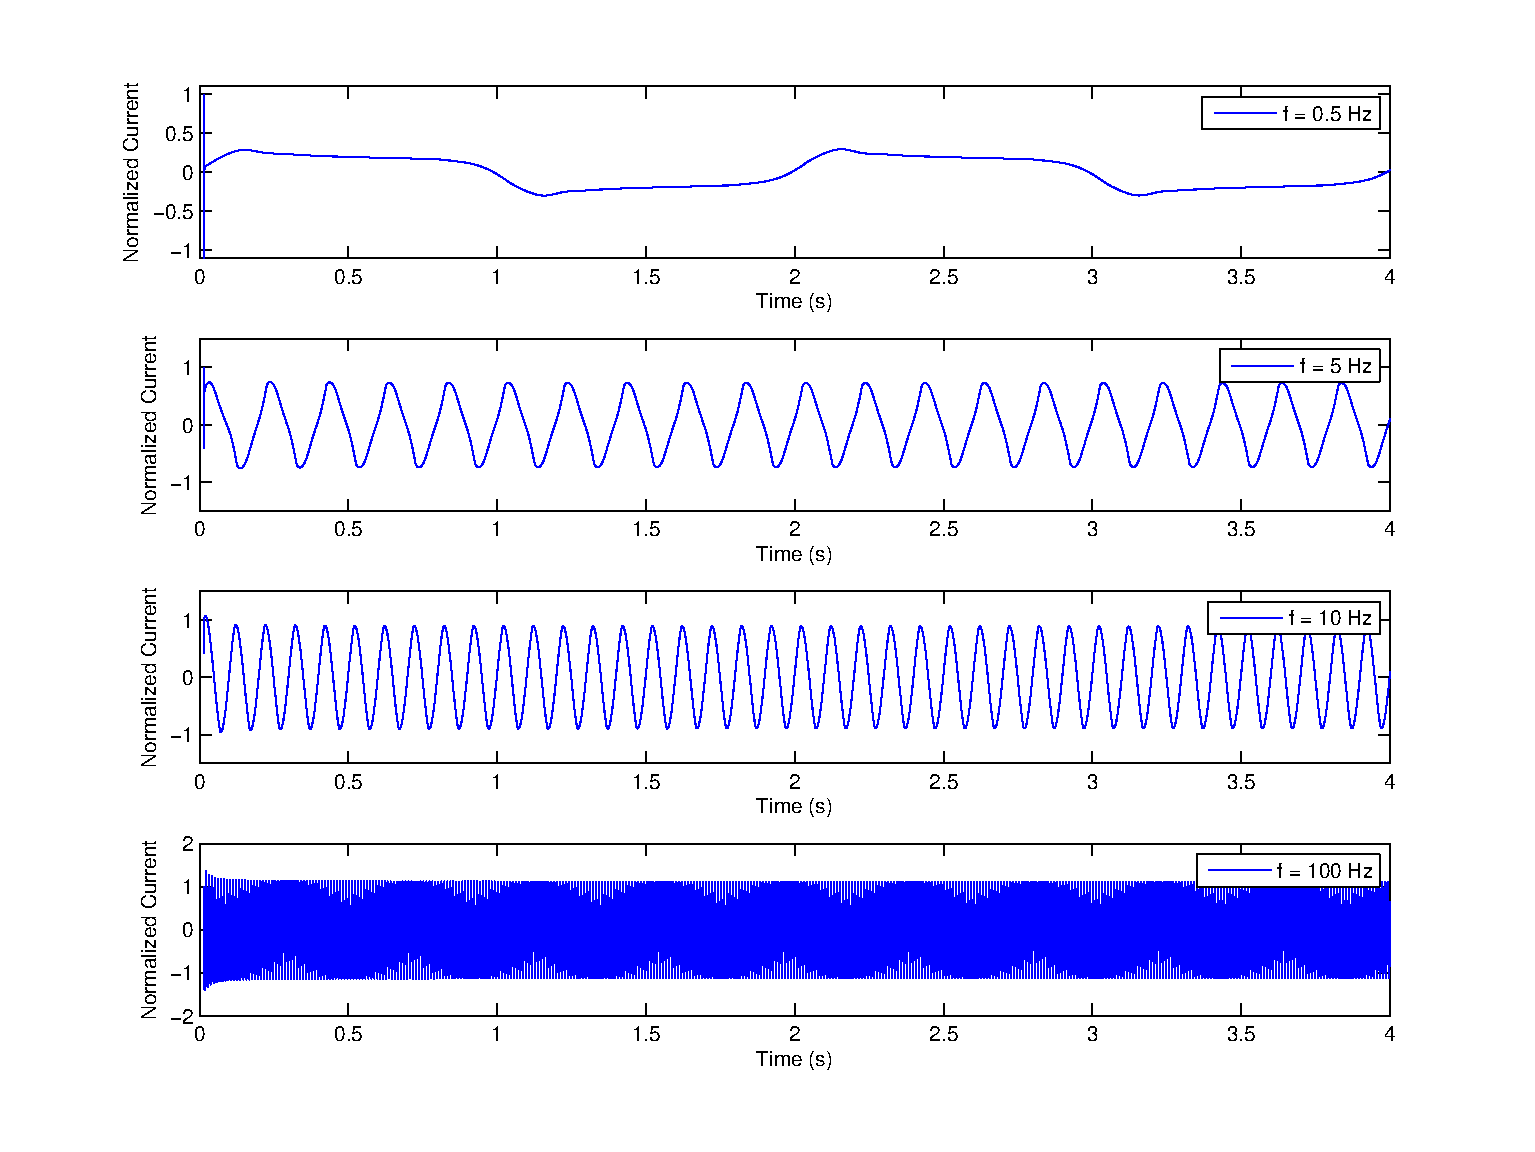
\includegraphics[scale=0.50]{2D_Memristor_Current_f}
\caption{} 
\label{}
\end{figure}

\begin{figure}[!htp]
\centering
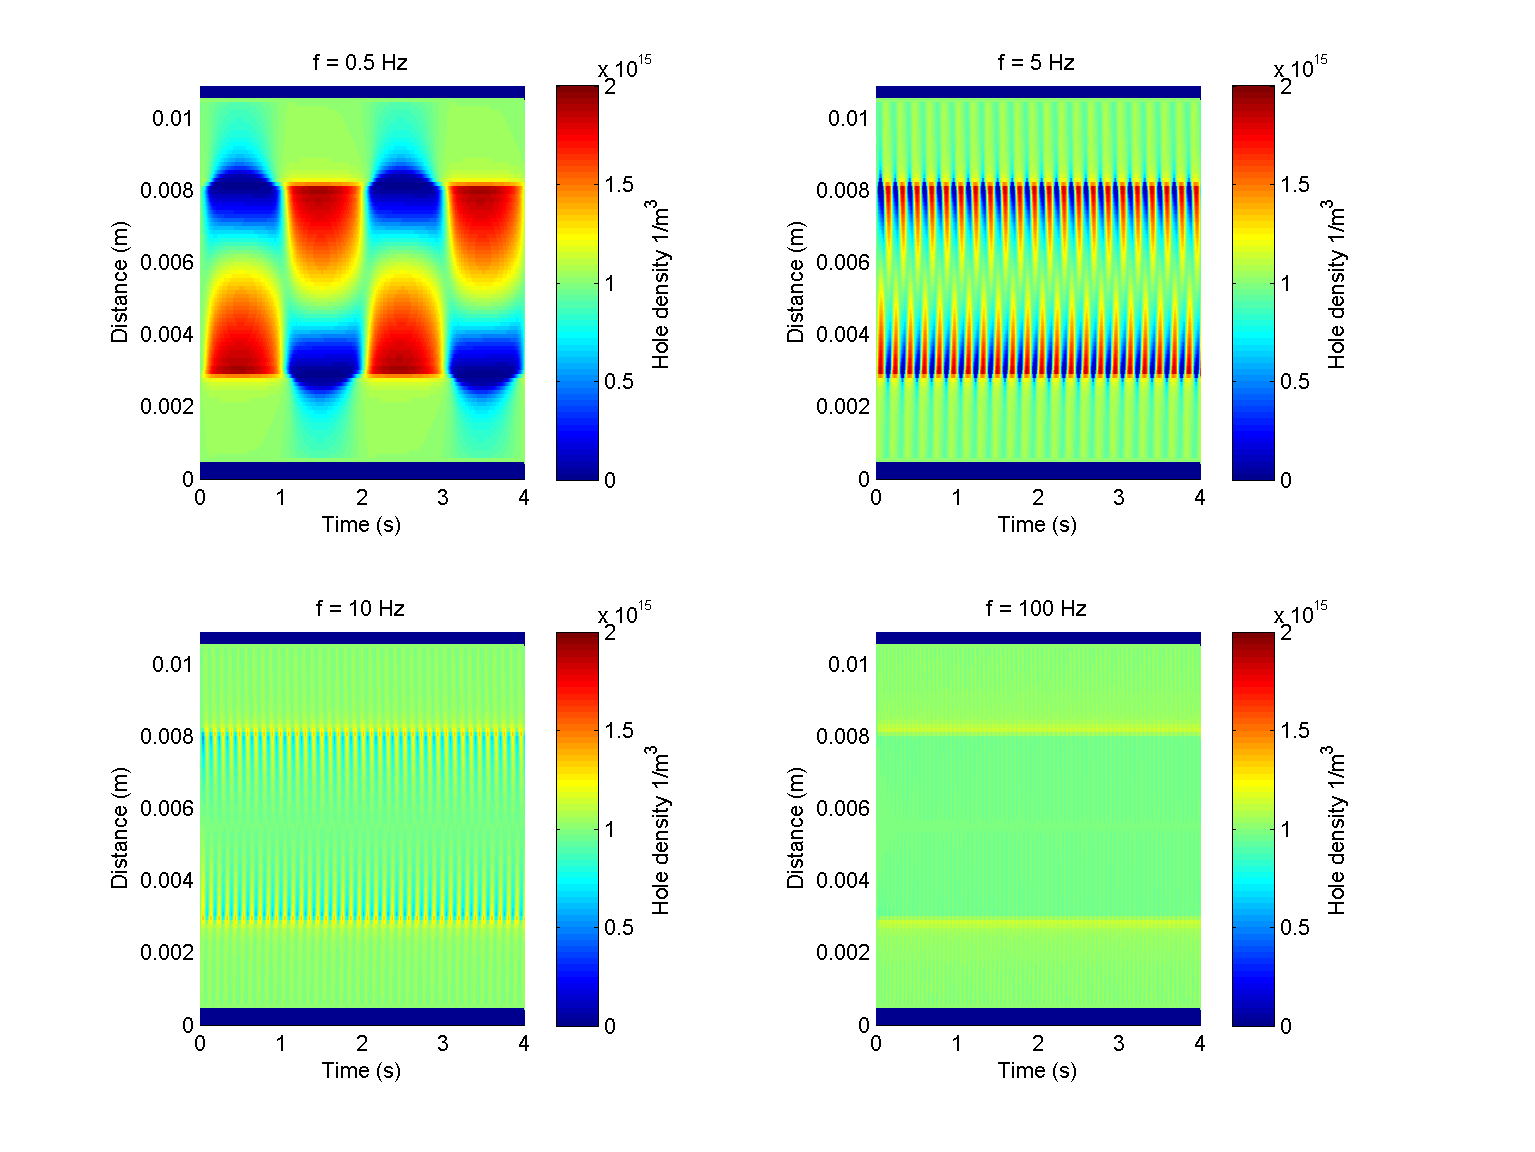
\includegraphics[scale=0.55]{2D_Memristor_f_Hole}
\caption{} 
\label{}
\end{figure}

\begin{figure}[!htp]
\centering
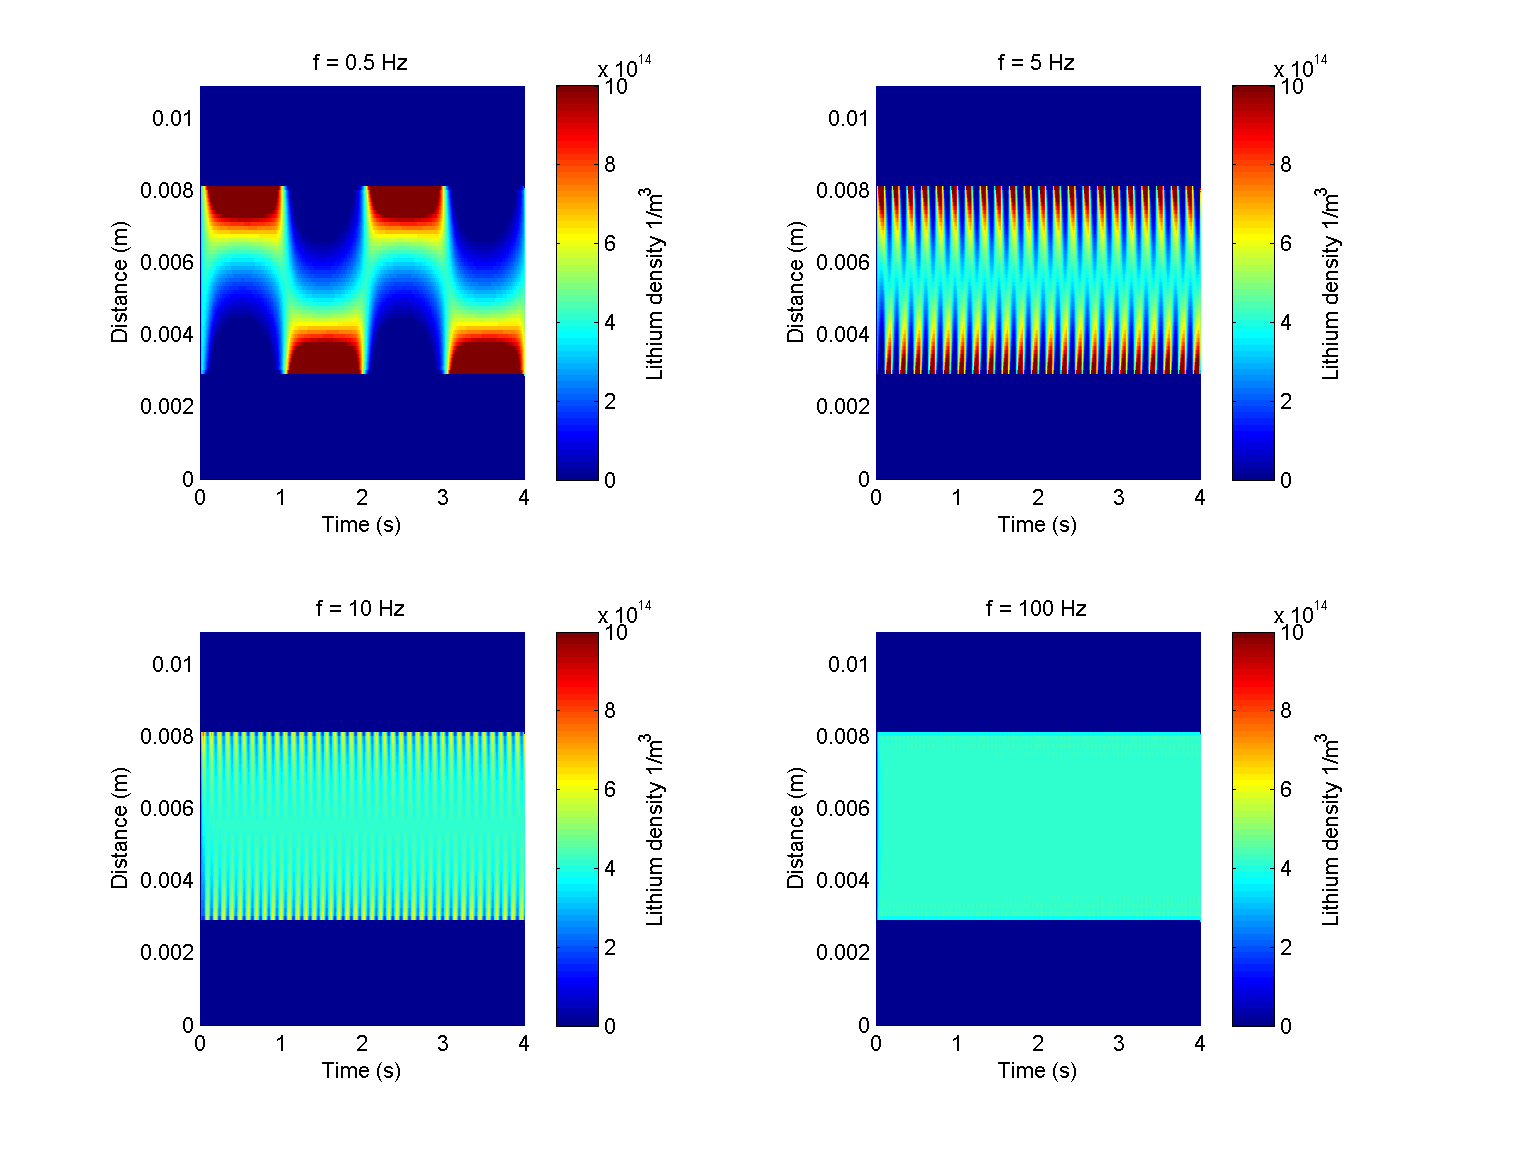
\includegraphics[scale=0.55]{2D_Memristor_f_Lithium}
\caption{} 
\label{}
\end{figure}

\begin{figure}[!htp]
\centering
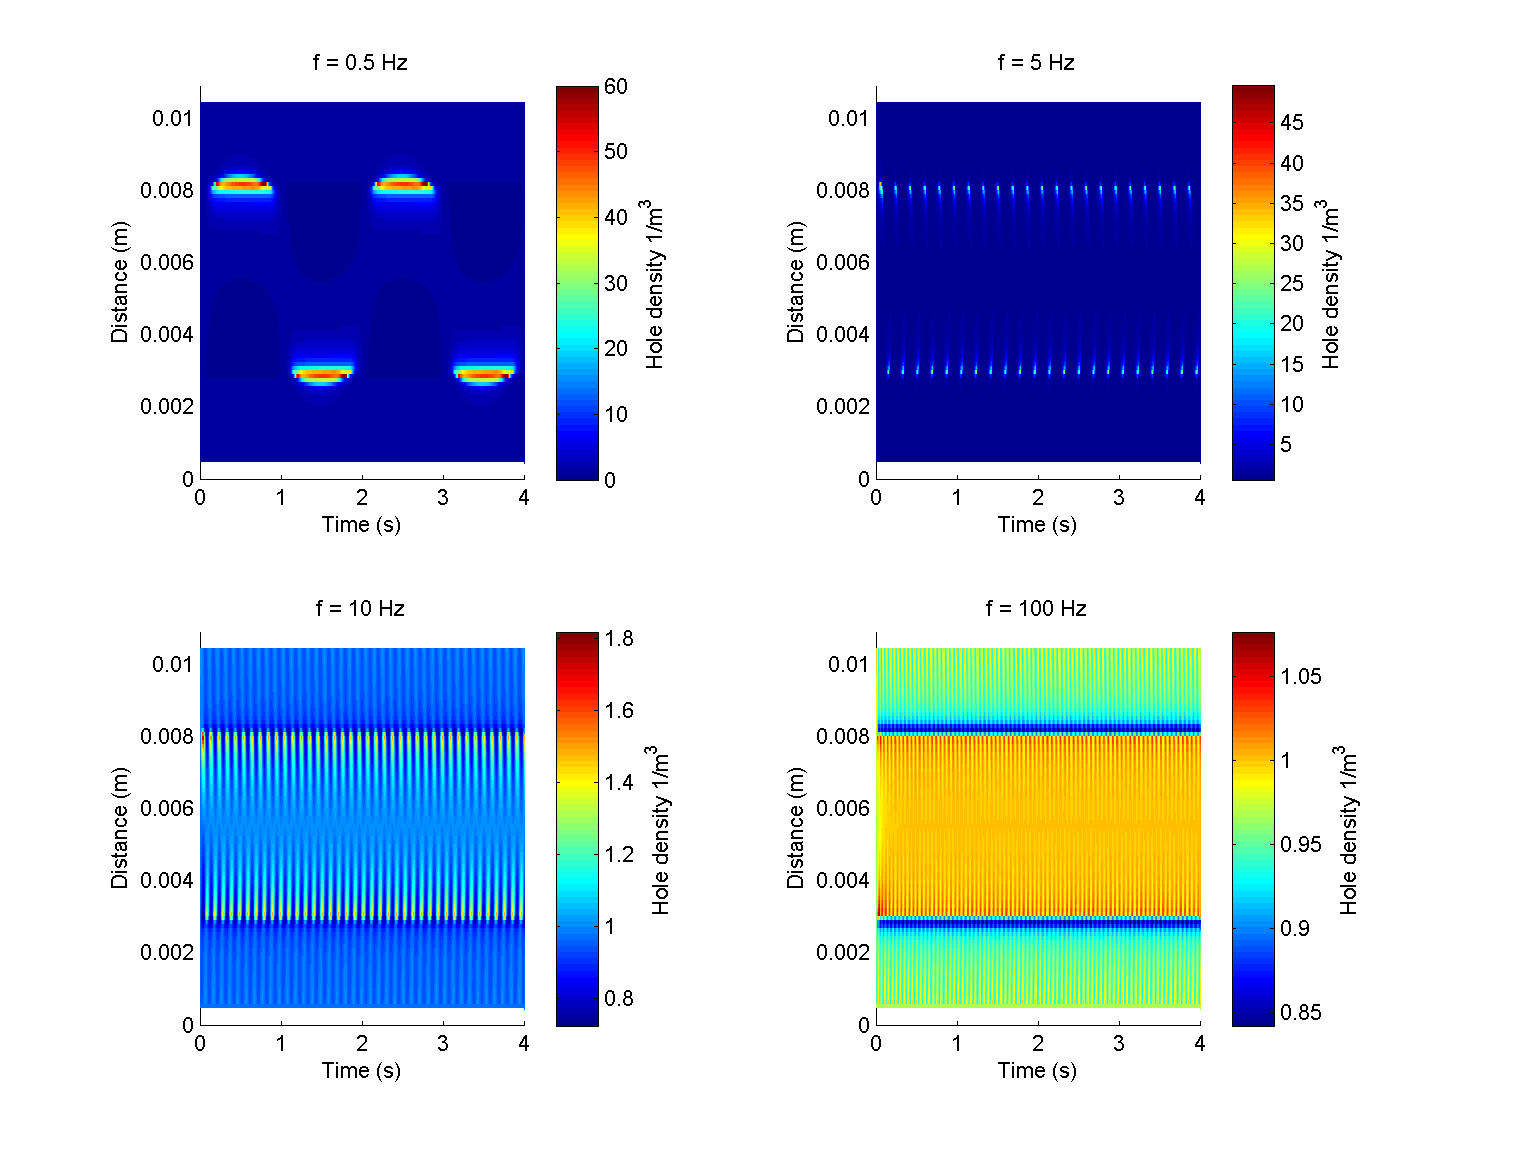
\includegraphics[scale=0.55]{2D_Memristor_f_Resistivity}
\caption{} 
\label{}
\end{figure}


\begin{figure}[!htp]
\centering
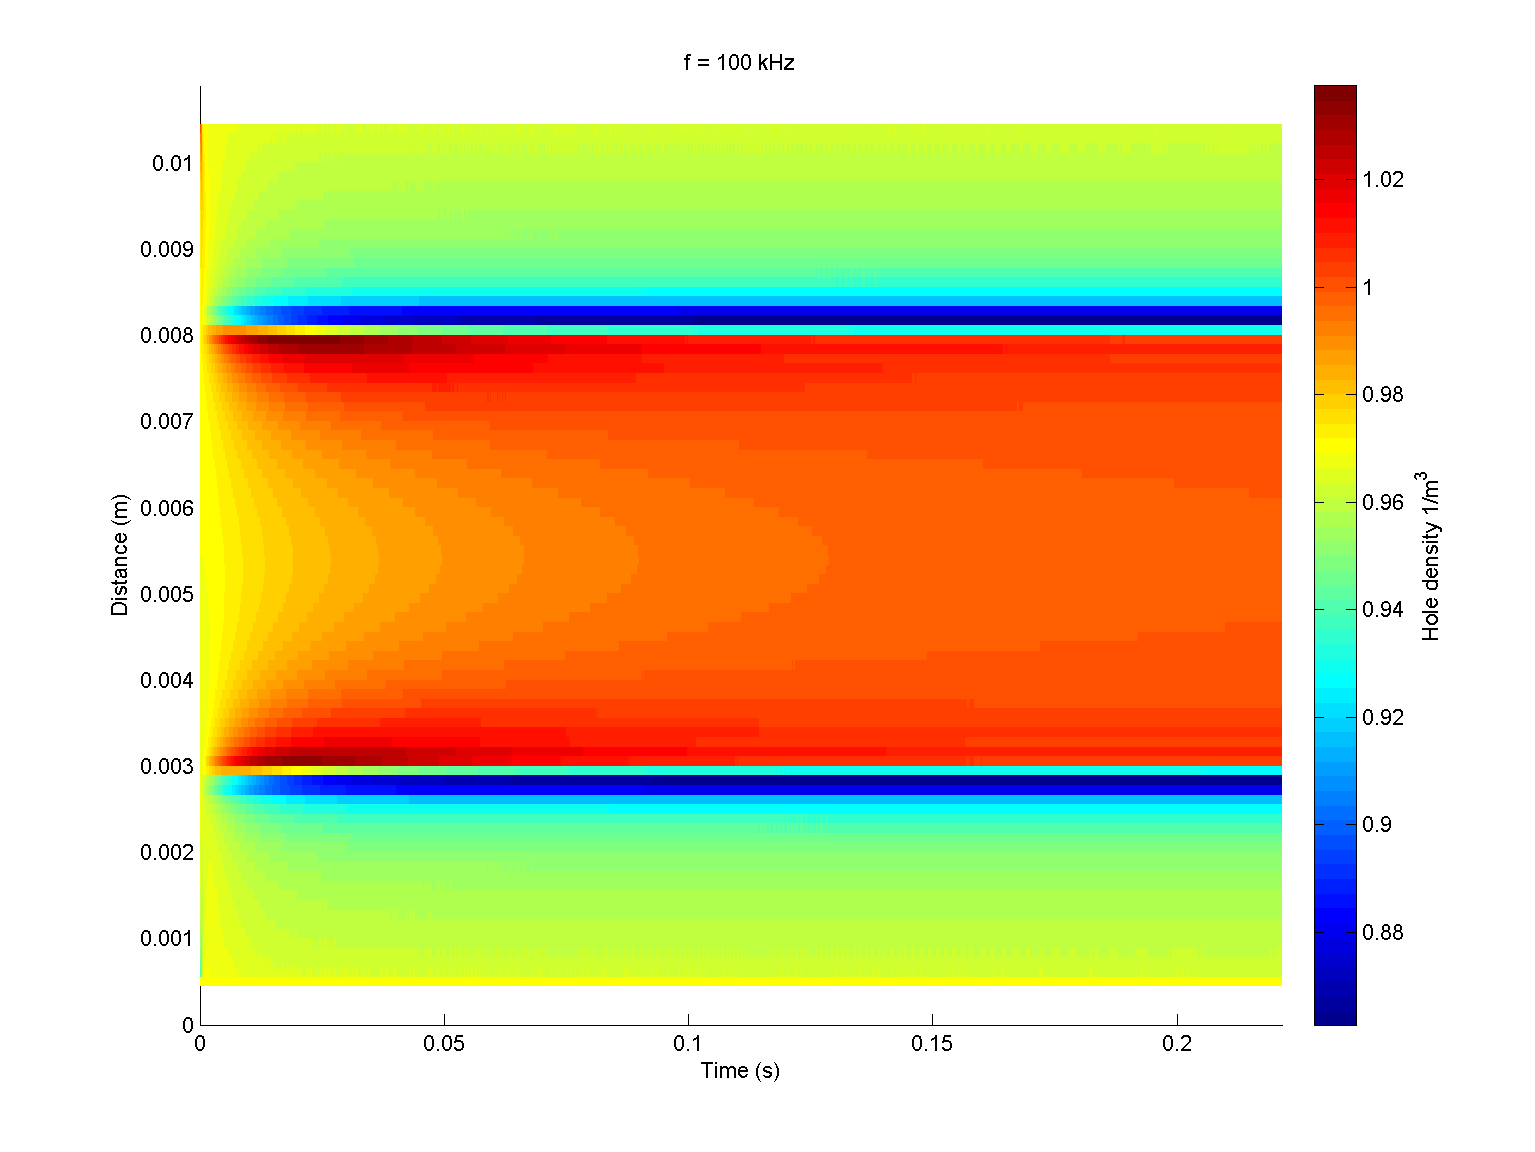
\includegraphics[scale=0.50]{2D_Memristor_f_Resistivity_1e5}
\caption{} 
\label{}
\end{figure}

\clearpage
\section{Experiment vs. Simulation}



\begin{figure}[!htp]
\centering
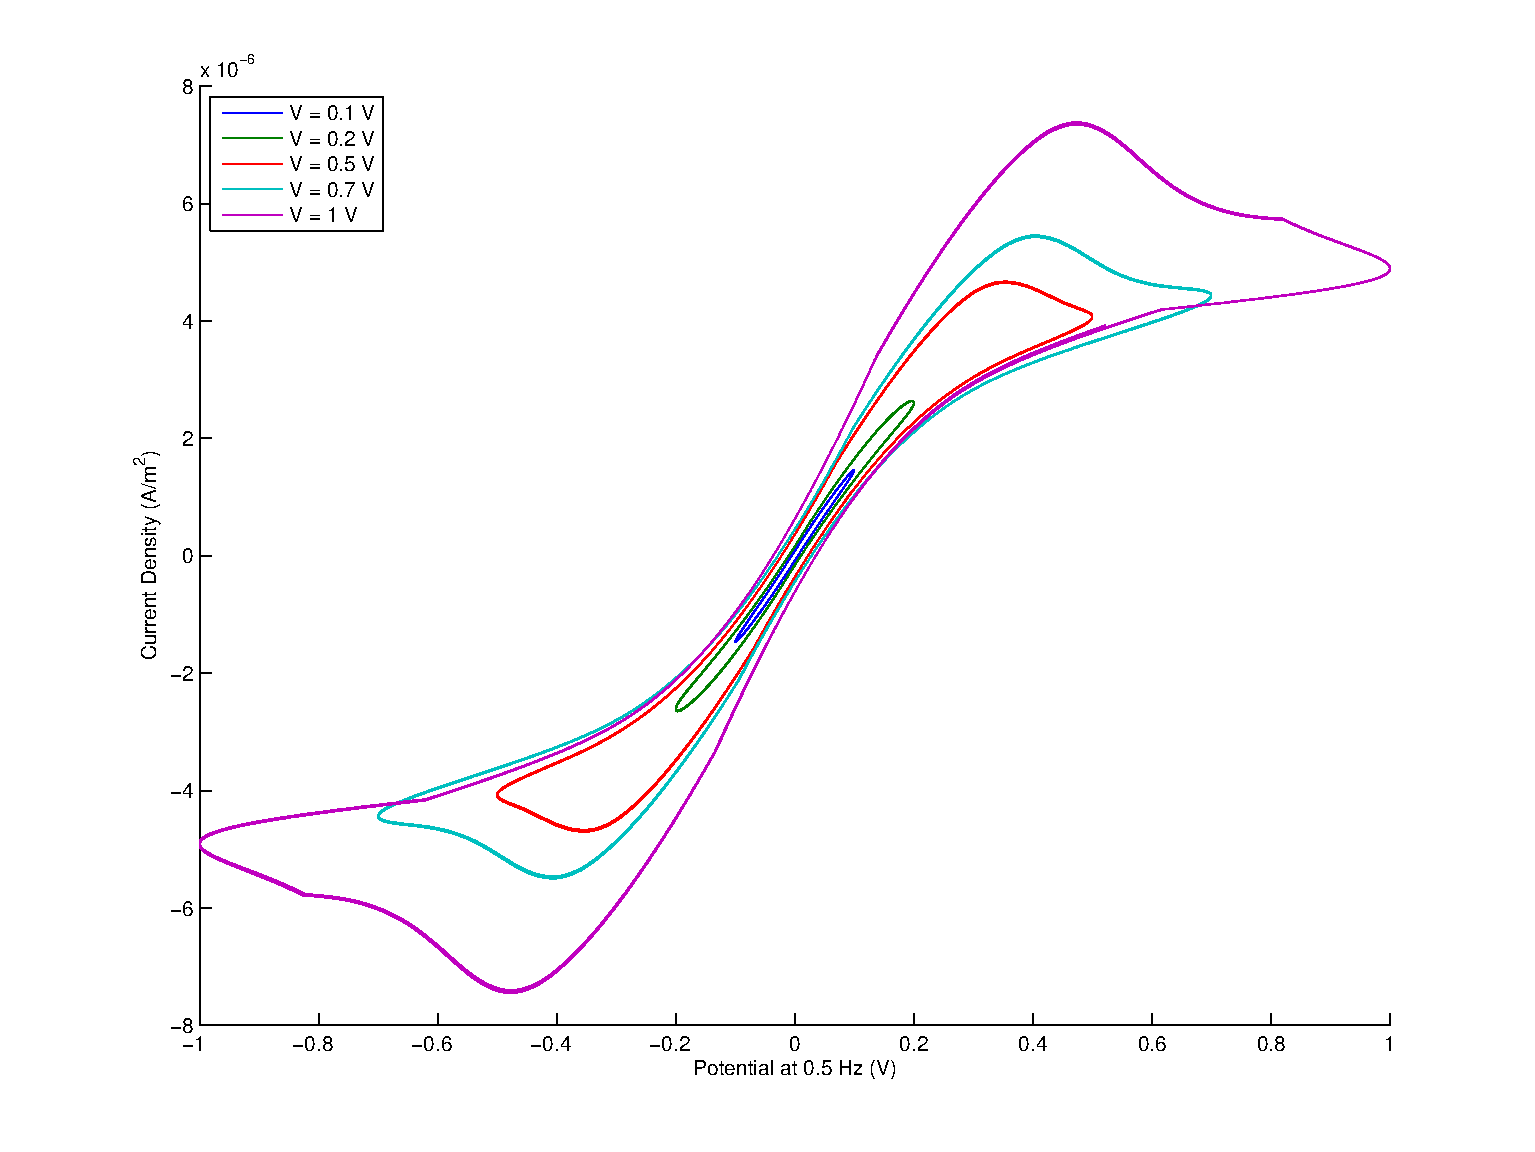
\includegraphics[scale=0.45]{2D_Memristor_5e-1Hz}
\caption{} 
\label{}
\end{figure}


\begin{figure}[!htp]
\centering
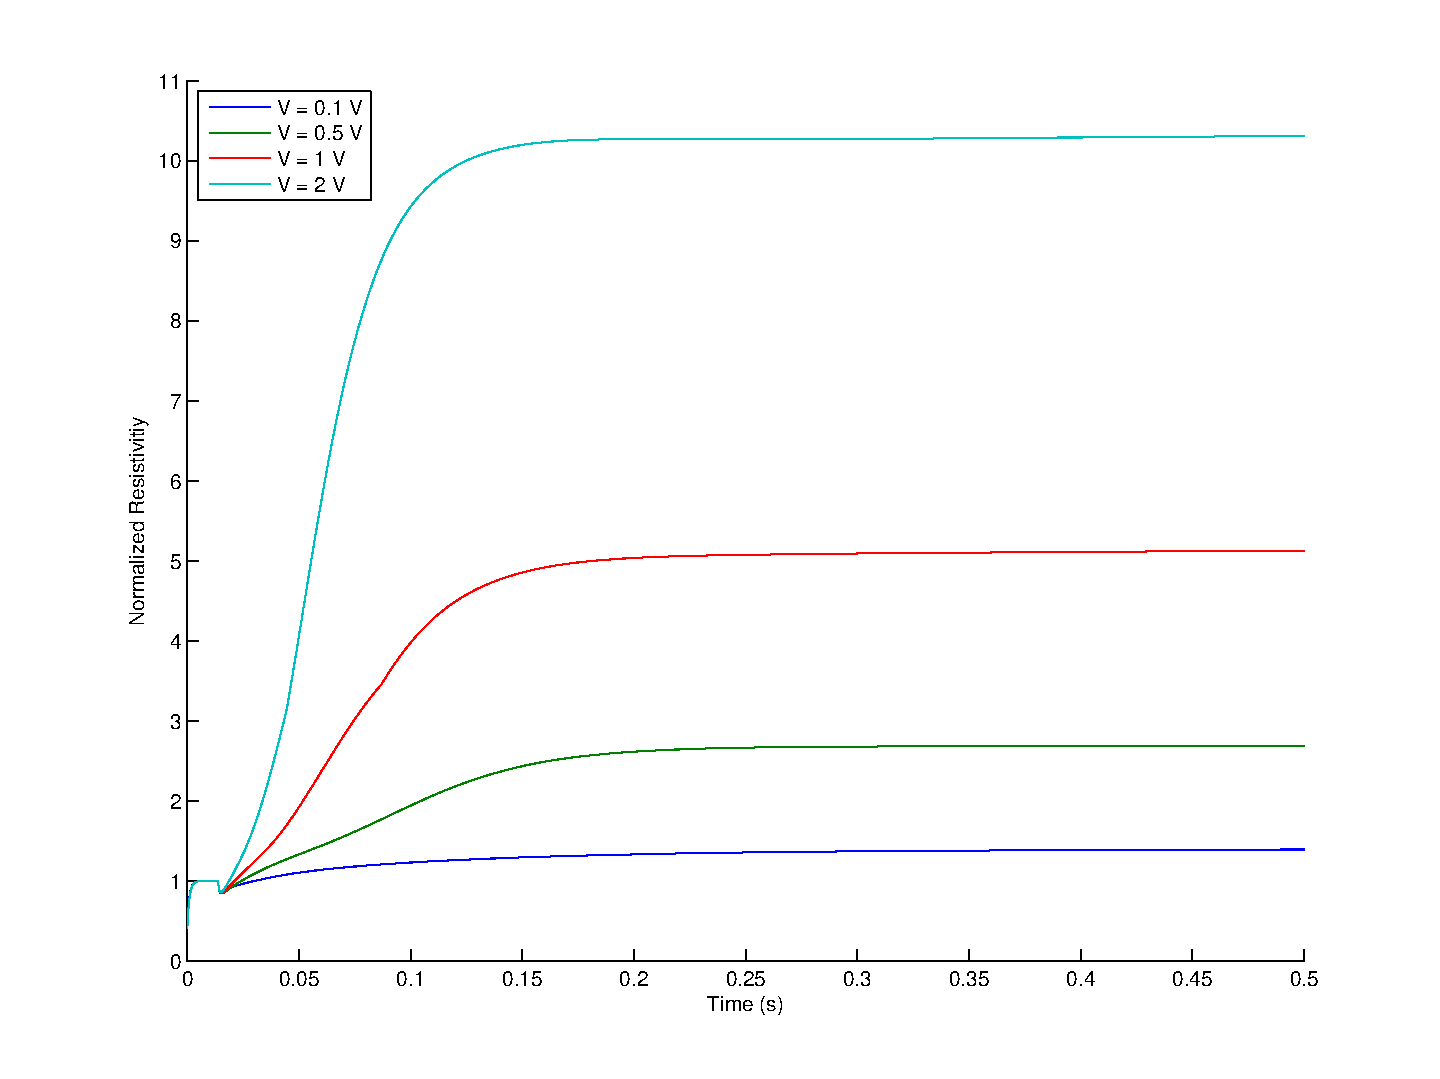
\includegraphics[scale=0.50]{2D_Memristor_V_chng}
\caption{} 
\label{}
\end{figure}
